\documentclass{scrartcl}
\usepackage{etex}
\usepackage[ngerman]{babel}
\usepackage[utf8]{inputenc}
\usepackage[T1]{fontenc}
\usepackage{amsmath, amssymb}
\usepackage{graphicx}

\usepackage{pgfplots}
\pgfplotsset{compat=1.11}
\usepgfplotslibrary{external}
\usepackage{pgfplotstable}

\usepackage{booktabs}
\usepackage{multirow}
\usepackage{longtable}
\usepackage{ulsy}
%\usepackage{pst-all}
\usepackage{picture}
\usepackage[automark]{scrpage2}
\usepackage{caption}
\pagestyle{scrheadings}
\ihead[]{Friedrich Hübner 2897111}
\ohead[]{Fiona Paulus 2909625} 

\author{Friedrich Hübner 2897111\\
Fiona Paulus 2909625}
\title{Computerphysik\\Hausarbeit 3\\Aufgabe 5}

\begin{document}
\maketitle
\newpage

\section*{Allgemeine Hinweise}
Zu a):\\
Das Programm wurde unter Windows 10 mit "g++ -o abgabe3\_5\_bessel.exe -Wall -Wextra -std=c++0x -O2 -static abgabe3\_5\_bessel.cpp"\;kompiliert.\\
Das Programm wird gestartet mit 'abgabe3\_5\_bessel n l r', wobei $n \in \mathbb{N}$ der Parameter der Besselfunktion ist und $l,r$ das Intervall, auf dem die Besselfunktion berechnet werden soll.\\

Zu b):\\
Das Programm wurde unter Windows 10 mit "g++ -o abgabe3\_5.exe -Wall -Wextra -std=c++0x -O2 -static abgabe3\_5.cpp"\;kompiliert.\\
Das Programm wird gestartet mit 'abgabe3\_5'. 

\section*{a) (abgabe3\_5\_bessel.cpp)}
Der Funktionswert der Besselfunktion wird mithilfe der zusammengesetzten Trapezformel berechnet. Im Intervall (l,r) wird an 1000 gleichverteilten x-Werten der Funktionswert berechnet und ausgegeben.

\begin{center}
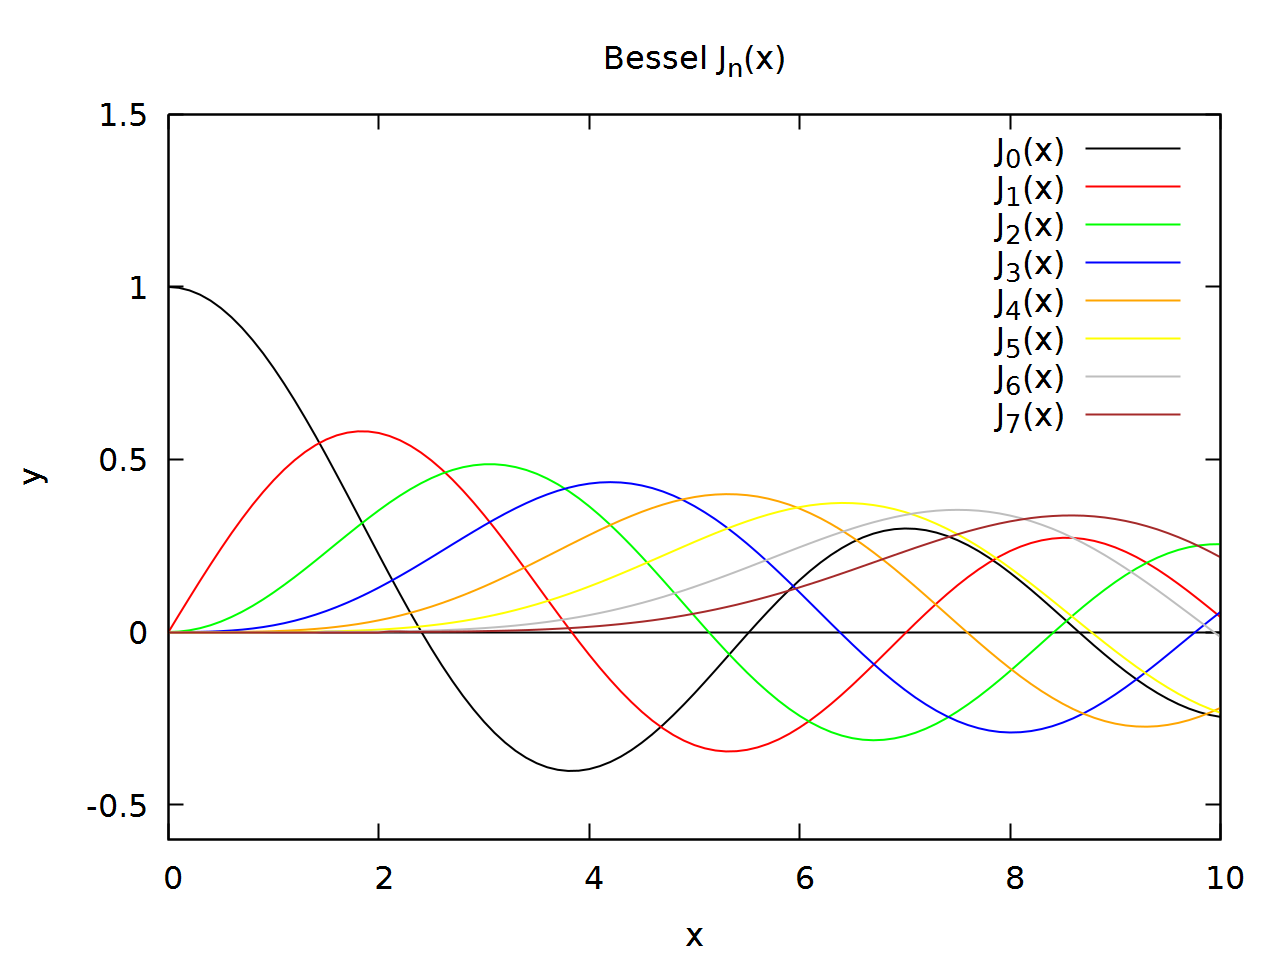
\includegraphics[scale=0.3]{plot_bessel.png}
\captionof{figure}{Die ersten 8 Besselfunktionen}
\end{center}

\section*{b) (abgabe3\_5.cpp)}
Zur Berechnung der Besselfunktion wird der Algorithmus aus a) verwendet.\\
Es wird einfach die Formel in der Aufgabenstellung bei mehreren äquidistanten $\theta$ ausgewertet. Die Ausgabe erfolgt in slit.txt\\

Dabei ergibt sich folgendes Bild:\\
\begin{center}
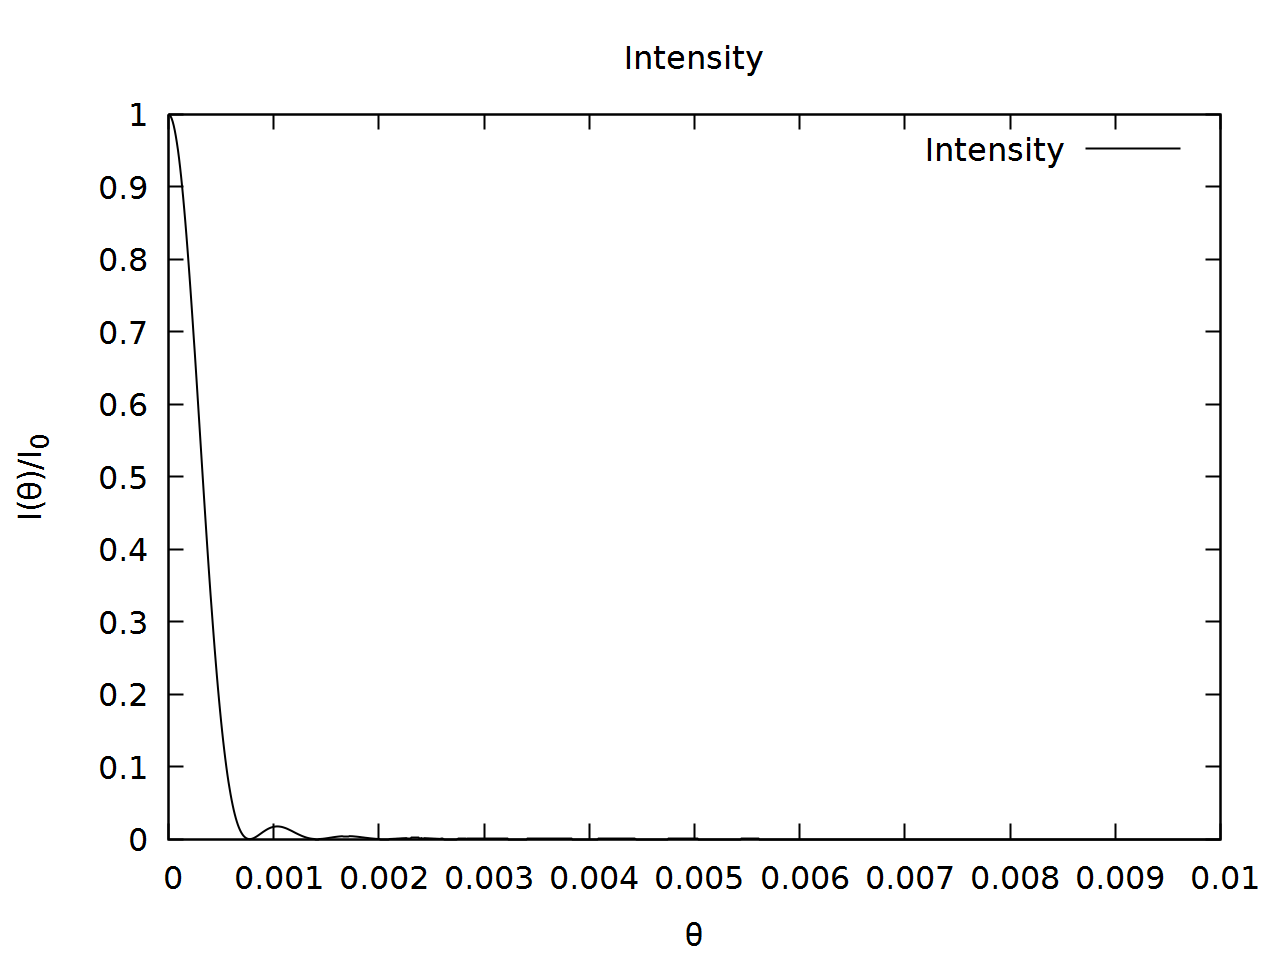
\includegraphics[scale=0.3]{plot_slit.png}
\captionof{figure}{Beugungsbild an einer Kreisblende}
\end{center}
\begin{center}
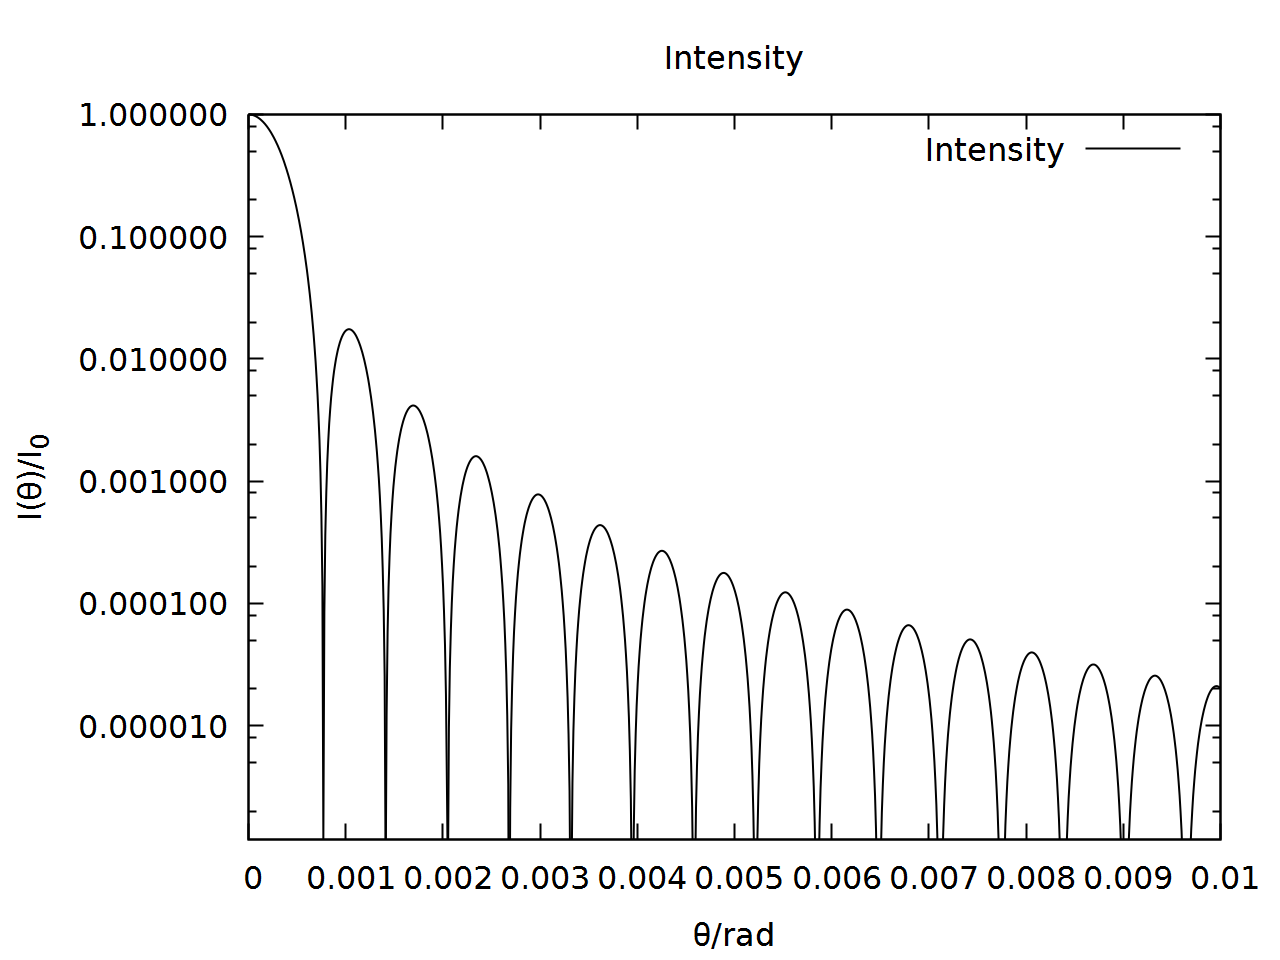
\includegraphics[scale=0.3]{plot_slit_log.png}
\captionof{figure}{Beugungsbild an einer Kreisblende (logarithmisch)}
\end{center}

\section*{c) (abgabe3\_5.cpp)}
Im selben Programm werden auch noch Maxima und Minima bestimmt. Dazu werden alle Werte durchgegangen. Ist ein Wert sowohl größer als der Vorgänger als auch der Nachfolger, so ist an dieser Stelle ein Maxmimum. Für Minima ist es analog. Man speichert sich zunächst nur den Index des Punktes, an dem die Extremstelle vorliegt und berechnet später daraus den Winkel.\\
Dabei ergeben sich folgende Maxima und Minima:\\
\begin{center}
\captionof{table}{Maxima}
\begin{tabular}{ccc}
\toprule
n & $\theta/rad$ & $I(\theta)/I_0$\\
\midrule
0 & 0 & 1\\
1 & 0.00103103 & 0.0174927\\
2 & 0.00169169 & 0.00415657\\
3 & 0.00234234 & 0.0016005\\
4 & 0.00298298 & 0.000779314\\
5 & 0.00361361 & 0.000436851\\
6 & 0.00425425 & 0.000269287\\
7 & 0.00488488 & 0.000177494\\
8 & 0.00552553 & 0.00012319\\
9 & 0.00615616 & 8.89594e-005\\
10 & 0.00678679 & 6.6293e-005\\
\bottomrule
\end{tabular}
\end{center}

\begin{center}
\captionof{table}{Minima}
\begin{tabular}{ccc}
\toprule
n & $\theta/rad$\\
\midrule
1 & 0.000770771\\
2 & 0.00141141\\
3 & 0.00205205\\
4 & 0.00268268\\
5 & 0.00331331\\
6 & 0.00395395\\
7 & 0.00458458\\
8 & 0.00521522\\
9 & 0.00584585\\
10 & 0.00648649\\
\bottomrule
\end{tabular}
\end{center}

\section*{Sonstige abgegebene Dateien}
\subsection*{plot\_bessel.plt}
Die Plot-Datei für die Besselfunktionen
\subsection*{plot\_slit.plt}
Die Plot-Datei für die Kreisblende
\subsection*{slit.txt}
Enthält die Plotdaten für die b)

\end{document}